\documentclass[a4paper,12pt]{article}
%%%%%%%%%%%%%%%%%%%%%%%%%%%%%%%%%%%%%%%%%%%%%%%%%%%%%%%%%%%%%%%%%%%%%%%%%%%%%%%%%%%%%%%%%%%%%%%%%%%%%%%%%%%%%%%%%%%%%%%%%%%%%%%%%%%%%%%%%%%%%%%%%%%%%%%%%%%%%%%%%%%%%%%%%%%%%%%%%%%%%%%%%%%%%%%%%%%%%%%%%%%%%%%%%%%%%%%%%%%%%%%%%%%%%%%%%%%%%%%%%%%%%%%%%%%%
\usepackage{eurosym}
\usepackage{vmargin}
\usepackage{amsmath}
\usepackage{graphics}
\usepackage{epsfig}
\usepackage{framed}
\usepackage{subfigure}
\usepackage{fancyhdr}

\setcounter{MaxMatrixCols}{10}
%TCIDATA{OutputFilter=LATEX.DLL}
%TCIDATA{Version=5.00.0.2570}
%TCIDATA{<META NAME="SaveForMode"CONTENT="1">}
%TCIDATA{LastRevised=Wednesday, February 23, 201113:24:34}
%TCIDATA{<META NAME="GraphicsSave" CONTENT="32">}
%TCIDATA{Language=American English}

\pagestyle{fancy}
\setmarginsrb{20mm}{0mm}{20mm}{25mm}{12mm}{11mm}{0mm}{11mm}
\lhead{MA4128} \rhead{Kevin O'Brien} \chead{Week 8 Part B} %\input{tcilatex}

%http://www.electronics.dit.ie/staff/ysemenova/Opto2/CO_IntroLab.pdf
\begin{document}

\tableofcontents
\newpage

\section{Output of Linear Regression Analysis}
Linear regression is used when you want to predict the value of a variable based on the value of another variable. The variable we want to predict is called the dependent variable (or sometimes, the outcome variable). The variable we are using to predict the other variable's value is called the independent variable (or sometimes, the predictor variable).
\[ \hat{y} = b_o + b_1 x \]
\begin{itemize}
\item $b_o$ is the intercept estimate
\item $b_1$ is the slope estimate
\item $\hat{y}$ is the \textbf{\textit{fitted}} y-value, given a specified value of the indepenent variable $x$.
\item The fitted value and the observed value of y often differ. This difference is known as the \textbf{\textit{residual}}
\end{itemize}

For example, you could use linear regression to understand whether exam performance can be predicted based on revision time; whether cigarette consumptions can be predicted based on smoking duration; and so forth. If you have two or more independent variables, rather than just one, you need to use \textbf{\textit{multiple regression}}.

SPSS will generate quite a few tables of output for a linear regression procedure. Only the three main tables required to understand your results from the linear regression procedure, assuming that no assumptions have been violated.

This includes relevant scatterplots, histogram (with superimposed normal curve) and Normal P-P Plot, and case-wise diagnostics and Durbin-Watson statistic tables. Below, we focus on the results for the linear regression analysis only.

\begin{figure}[h!]
\begin{centering}
  % Requires \usepackage{graphicx}
  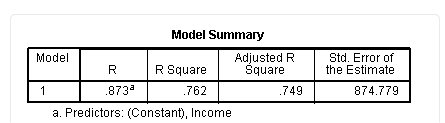
\includegraphics[width=10cm]{Regre4.jpg}\\
  \caption{Model Summary table}
\end{centering}
\end{figure}

The first table of interest is the \textbf{\textit{Model Summary}} table. This table provides the R and $R^2$ value. The R value is 0.873, which represents the simple correlation. It indicates a high degree of correlation. The $R^2$ value indicates how much of the dependent variable, \textbf{\textit{price}} (Not evident on output), can be explained by the independent variable,\textbf{\textit{income}}. In this case, 76.2\% can be explained, which is very large.


The next table is the ANOVA table. This table indicates that the regression model predicts the outcome variable significantly well. How do we know this? Look at the \textbf{\textit{Regression}} row and go to the \textbf{Sig.} column. This indicates the statistical significance of the regression model that was applied. Here,the p-value is  $p < 0.0005$, which is less than 0.05, and indicates that, overall, the model applied can statistically significantly predict the outcome variable.

\begin{figure}[h!]
\begin{centering}
  % Requires \usepackage{graphicx}
  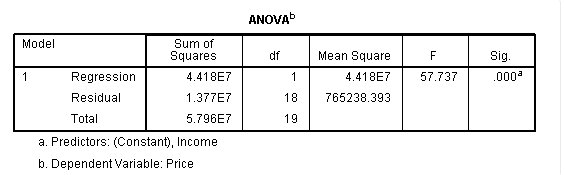
\includegraphics[width=10cm]{Regre5.jpg}\\
  \caption{ANOVA Table}
\end{centering}
\end{figure}

The next table again, \textbf{\textit{Coefficients}}, provides us with information on each predictor variable. This gives us the information we need to predict price from income. We can see that both the constant and income contribute significantly to the model (by looking at the Sig. column). By looking at the B column under the Unstandardized Coefficients column, we can present the regression equation as:

\textit{\textbf{ $\hat{Price}$ = 8287 + 0.564(Income)}}

\begin{figure}[h!]
\begin{centering}
  % Requires \usepackage{graphicx}
  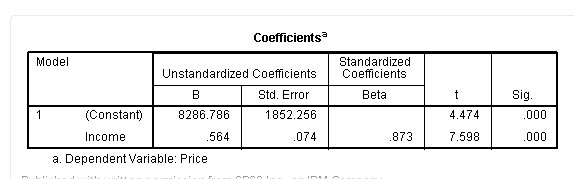
\includegraphics[width=10cm]{Regre6.jpg}\\
  \caption{Coefficients Table}
\end{centering}
\end{figure}


\newpage
\section{Multiple Linear Regression}
\subsection{What is Multiple Linear Regression}

Multiple regression is a statistical technique that allows us to predict a numeric value on the response variable on the basis of the observed values on several other independent variables.


\[\hat{y} = b_0 + b_1x_1 + b_2x_2 + \ldots \]

\begin{itemize}
\item $\hat{y}$ is the \textbf{\textit{fitted value}} for the dependent variable \textbf{$Y$}, given a linear combination of values for the independent valriables.

\item $x_i$ is the value for independent variable \textbf{$X_i$}. (For Example, $x_1$ is the value for independent variable \textbf{$X_1$}.)
\item $b_o$ is the constant regression estimate ( commonly known as the \textbf{Intercept Estimate} in the case of simple linear regression).
\item $b_i$ is the regression estimate for Independent Variable \textbf{$X_1$} ( commonly known as the \textbf{Slope Estimate} in the case of simple linear regression).
\end{itemize}

\subsubsection{Simple Example}
Suppose we were interested in predicting how much an individual enjoys their job. Independent Variables such as salary, extent of academic qualifications, age, sex, number of years in full-time employment and socioeconomic status might all contribute towards \textbf{\textit{job satisfaction}}.

If we collected data on all of these variables, perhaps by surveying a few hundred members of the public, we would be able to see how many and which of these variables gave rise to the most accurate prediction of job satisfaction. We might find that job satisfaction is most accurately predicted by type of occupation, salary and years in full-time employment, with the other variables not helping us to predict job satisfaction.

\subsection{Variable Selection}
Often we require the optimal set of independent variables to adequately describe the data, without overfitting. As such we will use variable selection procedures. In statistical methods, the order in which the predictor variables are entered into (or taken out of) the model is determined according to the strength of their correlation with the response variable. Actually there are several versions of this method, called forward selection, backward selection and stepwise selection.

The main procedures are as follows:
\begin{itemize}
\item Forward Selection
\item Backward Elimination
\item Stepwise Selection
\end{itemize}

The essential concept is the estimation of the relationship between a predictor
variable and a response variable after controlling for the effects of other
predictors in the equation. One such estimate is the semi-partial correlation coefficient.

\subsection{Variable Selection Procedures in SPSS}

\begin{itemize}
\item \textbf{Enter}: This is the forced entry option. SPSS will enter at one time all specified variables regardless of significance levels.
\item \textbf{Forward}: This method will enter variables one at a time, based on the significance value to enter.
\item \textbf{Backward}: This enters all independent variables at one time and then removes variables one at a time based on a preset significance value to remove.
\item \textbf{Stepwise}: This combines both forward and backward procedures. Since inter correlations are complex, the variance due to certain variables will change when new variables are entered into the equation. This is the most frequently used of the regression methods.
\item \textbf{Remove}: This is the forced removal option. It requires an initial regression analysis usingthe Enter procedure. In the next block (Block 1 of 1) you may specify one or morevariables to remove. SPSS will then remove the specified variables and run the analysis again.
\end{itemize}

There are different ways that the relative contribution of each predictor variable can be assessed. In the ``simultaneous" method (which SPSS calls the Enter method), the researcher specifies the set of predictor variables that make up the model. The success of this model in predicting the criterion variable is then assessed.

%In contrast, ``hierarchical" methods enter the variables into the model in a specified order. The order specified should reflect some theoretical consideration or previous
%findings. If you have no reason to believe that one variable is likely to be more important than another you should not use this method. As each variable is entered into the model its contribution is assessed. If adding the variable does not significantly increase the predictive power of the model then the variable is
%dropped.

\subsection{Forward Selection}
We consider first forward Selection.In Forward selection, SPSS enters the variables into the model one at a time in an
order determined by the strength of their correlation with the response variable. The effect of adding each is assessed as it is entered, and variables that do not significantly add to the success of the model are excluded.

In this procedure, once a predictor is selected into the model, it cannot be removed. Other predictors may be added at future steps, but predictors already in the model remain in the model. As we will see, this is in contrast to SPSS's stepwise regression, in which we can specify criteria for both adding and removing predictors at each step.

\subsection{Steps in Forward Selection}
\textbf{Step 1}\\
Firstly, the predictor variable with the largest squared correlation with the dependent variable Y is entered into the model. Since this is the first step of the selection procedure, entering the predictor with the largest squared correlation is equivalent to entering the predictor with the \textbf{largest squared semi-partial} correlation. 

It may seem trivial to bring up the idea of semi-partial correlation at step 1 of the procedure, but we do so because at subsequent steps, the criterion for entrance into the regression equation will be the squared semi-partial correlation (or equivalently, the amount of variance contributed by the new predictor over and above variables already entered into the equation).

\textbf{Step 2}\\
The unselected predictor variable with the largest squared semi-partial correlation with the dependent variable (hence referred to as $Y$) is selected. That is, the predictor with the largest correlation with $Y$ after being adjusted for the first predictor, is entered if it meets entrance criteria in terms of preset statistical significance for entry, what SPSS refers to as
\textbf{\texttt{PIN}} (probability of entry) criteria. 
It is important to note that even once this new predictor is entered at step 2, the predictor entered at step 1 remains in the equation, even if it's new semi-partial correlation with $Y$ is now less than what it was at step 1. 

This is the nature of the forward selection procedure, it does not re-evaluate already-entered predictors into the model after adding new variables. That is, it only add predictors to the model. 

%Again, this is in contrast to SPSS’s stepwise procedure (to be discussed in some detail shortly) in which in addition to entrance criteria being specified for new variables, removal criteria is also specified at each stage of the variable-selection procedure.
\textbf{Step 3}\\
The next unselected predictor with the largest squared semi-partial correlation with $Y$ is then selected. That is, the predictor with the largest correlation with Y after being adjusted for both of the first two predictors is entered. 

Selection for entrance of this variable is conditional upon its relationship with the previously entered variables at step 1 and step 2. Hence, for a variable to be entered at step 3, SPSS asks the question, \textit{"Which among available variables currently not entered into the regression equation contribute most to variance explained in Y given that variables entered at steps 1 and 2 remain in the model?"} Translated into statistical language, what this question boils down to is selecting the variable that has the largest statistically significant squared semi-partial correlation with Y.

\textbf{Subsequent Steps } \\
We do not detail subsequent steps for the reason that they mimic the preceding steps. It is worth noting that we didn't even really need to detail steps 2 and 3, and could have just stated the "rule" of forward regression by referring to the first step alone. 

We can state the general rule of forward regression as follows:
\begin{quote}
Forward regression, at each step of the selection procedure from step 1 through subsequent steps, chooses the predictor variable with the greatest squared semi-partial correlation with the response variable for entry into the regression equation. The given predictor will be entered if it satisfies entrance criteria (significance level, PIN) specified in advance by the researcher.
\end{quote}

The above is the simplest way to describe the procedural routine of how forward regression operates. What is perhaps most noteworthy about the above rule is what is not included just as much as what is included in the statement. Notice that nowhere in the rule is there any mention of removal of predictors at any step of the selection process. 

\subsection{Backward Selection}
In Backward selection, SPSS enters all the predictor variables into the model. The weakest predictor variable is then removed and the regression re-calculated. If this significantly weakens the model then the predictor variable is re-entered, otherwise it is deleted. This procedure is then repeated until only useful predictor variables remain in the model.

\subsection{Stepwise Selection}
Stepwise is the most sophisticated of these statistical methods. Each variable is entered in sequence and its value assessed. If adding the variable contributes to the model then it is retained, but all other variables in the model are then re-tested to see if they are still contributing to the success of the model. If they no longer contribute significantly they are removed. Thus, this method should ensure that you end up with the smallest possible set of predictor variables included in your model.

\subsection{The Remove Option}
In addition to the Enter, Stepwise, Forward and Backward methods, SPSS also offers the Remove method in which variables are removed from the model in a block - the use of this method will not be described here.

If you have no theoretical model in mind, and/or you have relatively low numbers
of cases, then it is probably safest to use Enter, the simultaneous method. Statistical
procedures should be used with caution and only when you have a large number of
cases. This is because minor variations in the data due to sampling errors can have a
large effect on the order in which variables are entered and therefore the likelihood
of them being retained. However, one advantage of the Stepwise method is that it
should always result in the most parsimonious model. This could be important if
you wanted to know the minimum number of variables you would need to measure
to predict the dependent variable. If for this, or some other reason, you decide to
select a statistical method, then you should really attempt to validate your results
with a second independent set of data. The can be done either by conducting a
second study, or by randomly splitting your data set into two halves . Only results that are common to both analyses should be reported.

\subsection{F values}

At each step, SPSS performs the following calculations: for each variable currently in the model, it computes the t-statistic for its estimated coefficient, squares it, and reports this as its \textbf{F-to-remove} statistic; for each variable not in the model, it computes the t-statistic that its coefficient would have if it were the next variable added, squares it, and reports this as its \textbf{F-to-enter} statistic.

At the next step, the program automatically enters the variable with the highest F-to-enter statistic, or removes the variable with the lowest F-to-remove statistic, in accordance with certain specified values. 

(Important: F = t-squared)

\subsection{Stepping Method Criteria}
Stepwise methods include or remove one independent variable at each step, based (by default) on the probability of F (p-value). The limits for the criteria controlling variable inclusion or removal can be specified by defining probabilities for \textbf{F-to-enter/F-to-remove} (or otherwise \textbf{values of F-to-enter/F-to-remove}, not recommended without a very thorough understanding of the F-distribution).




The following three stepwise methods are available.

\begin{itemize}
\item Stepwise Based on the p-value of F (probability of F), SPSS starts by entering the variable with the smallest p-value; at the next step again the variable (from the list of variables not yet in the equation) with the smallest p-value for F and so on. 
    
    Variables already in the equation are removed if their p-value becomes larger than the default limit due to the inclusion of another variable. The method terminates when no more variables are eligible for inclusion or removal.	
    
    This methods is based on both probability-to-enter (PIN) and probability to remove (POUT).
\item Backward Elimination: First all variables are entered into the equation and then sequentially removed. For each step SPSS provides statistics, namely $R^2$. At each step, the largest probability of F is removed (if the value is larger than POUT.
\item Forward Forward selection: at each step the variable not yet in the equation with the smallest probability of F is entered. as long as the value is smaller than PIN. The procedure stops when there are no variables that meet the entry criterion.
\end{itemize}
\newpage


\end{document}